%Part of/Parte di https://github.com/f-dinucci/appuntiMeccanicaFluidi/
%License/Licenza Creative Commons Attribution-ShareAlike 4.0 International (CC BY-SA 4.0) - attribution/attribuzione Francesco Di Nucci
%See also/Vedere anche https://creativecommons.org/licenses/by-sa/4.0/ and/e https://creativecommons.org/licenses/by-sa/4.0/legalcode
%
\section{Flusso lentamente variabile}
\subsection{Flusso in spazi stretti}
Nel caso di flusso lentamente variabile (alias flusso in spazi stretti) si vede che ci si può ricondurre alle equazioni di Stokes non solo in caso di Reynolds piccolo ma anche in determinate condizioni geometriche.
Si suppone di avere una geometria le cui dimensioni siano in questa relazione:
%
	\begin{equation*}
		\frac{h}{L} << 1
	\end{equation*}
%
%
	\begin{figure}[ht]
		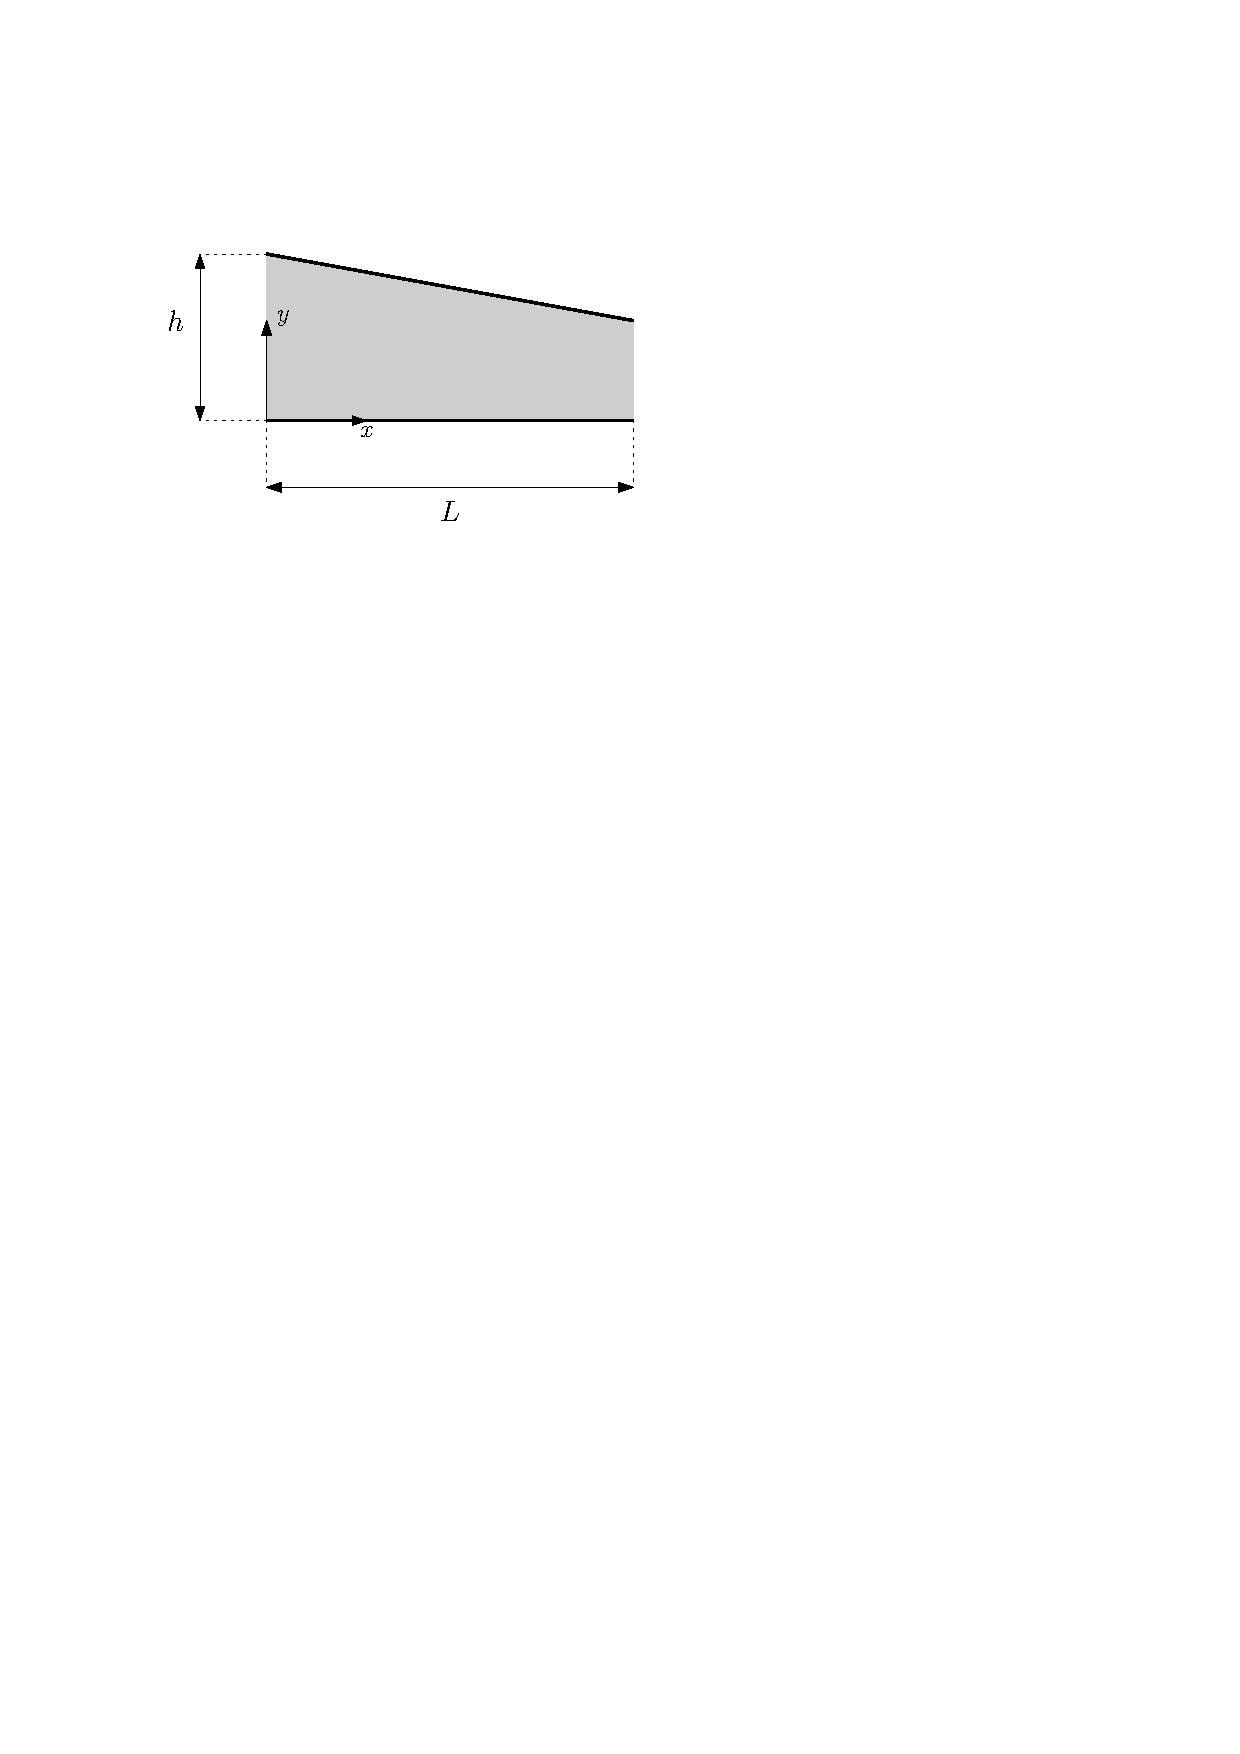
\includegraphics[scale=0.85]{./6.2 Flusso lentamente variabile/6.2-1}
		\centering
		\caption{Flusso lentamente variabile/in spazi stretti}
	\end{figure}
%
La relazione geometrica si riflette sugli ordini di grandezza delle derivate:
%
	\begin{equation*}
		\begin{gathered}
			\pdv{f}{y} >> \pdv{f}{x}\\
			\sim \frac{f_r}{h} \quad \sim \frac{f_r}{L}
		\end{gathered}
	\end{equation*} 
%

Per analizzare gli effetti gli ordini di grandezza conviene scrivere le equazioni per componenti, supponendo di trovarsi nel caso stazionario.
Si trova che $u_{xx}$ e $v_{xx}$ sono piccole:
%
	\begin{equation*}
		\begin{gathered}
			u_x + v_y = 0\\
			u u_x + v u_y + p_x = \frac{1}{R_e} (\cancel{u_{xx}} + u_{yy})\\
			u v_x + v v_y + p_y = \frac{1}{R_e} (\cancel{v_{xx}} + v_{yy})
		\end{gathered}
	\end{equation*} 
%
Affinché l'equazione di continuità abbia senso, ci si aspetta $\frac{v}{u} \sim \frac{h}{L}$.
Si introducono quindi $v$ ed $u$ di riferimento tali che:
%
	\begin{equation*}
		\frac{v_r}{u_r} = \frac{h}{L}
	\end{equation*}
%
Le equazioni diventano quindi:
%
	\begin{equation*}
		\begin{gathered}
			{\left( \frac{h}{L}\right)}^2 R_e (u u_x + v u_y) + \left( \frac{h}{L}\right) R_e p_x = u_{yy}\\
			{\left( \frac{h}{L}\right)}^2 R_e (u v_x + v v_y) + \left( \frac{h}{L}\right) R_e p_y = v_{yy}
		\end{gathered}
	\end{equation*} 
%
Si introduce poi la pressione di riferimento:
%
	\begin{equation*}
		\bar{p} = {\left( \frac{h}{L}\right)}^2  R_e p
	\end{equation*}
%
Per cui le equazioni diventano:
%
	\begin{equation*}
		\begin{gathered}
			{\left( \frac{h}{L}\right)}^2 R_e (u u_x + v u_y) + \bar{p}_x = u_{yy}\\
			{\left( \frac{h}{L}\right)}^2 R_e (u v_x + v v_y) +  \frac{L}{h} \bar{p}_y = v_{yy}
		\end{gathered}
	\end{equation*} 
%
A questo punto, se $\frac{h}{L} << 1$, anche $\frac{h^2}{L^2} << 1$, nella prima equazione si semplificano i termini non lineari.
Nella seconda invece $\frac{L}{h} >> 1$, conta solamente il termine moltiplicato per esso.
Mettendo assieme all'equazione di continuità le equazioni che descrivono il moto sono:
%
	\begin{equation*}
		\begin{gathered}
			\bar{p}_x = u_{yy}\\
			\bar{p}_y = 0\\
			u_x + v_y = 0
		\end{gathered}
	\end{equation*} 
%
Queste si sono ricavate da considerazioni geometriche sul condotto, il numero di Reynolds può anche essere grande, purché il raggruppamento $\frac{h^2}{L^2} R_e$ sia piccolo, è una condizione restrittiva sulla geometria, ma più permissiva sul numero di Reynolds.

\subsection*{Bibliografia 6.2}
\cite[Cap.\ 9.1]{PnueliGutfinger}
